\documentclass[10pt]{article}
\usepackage[utf8]{inputenc}
\usepackage[T1]{fontenc}
\usepackage{amsmath}
\usepackage{amsfonts}
\usepackage{amssymb}
\usepackage[version=4]{mhchem}
\usepackage{stmaryrd}
\usepackage{graphicx}
\usepackage[export]{adjustbox}
\graphicspath{ {./images/} }

\title{EXTRA MATHEMATICS ADMISSIONS TEST December 2020 \\
 Time allowed: 1 hour }

\author{}
\date{}


\begin{document}
\maketitle
\begin{center}
\begin{tabular}{|l|l|}
\hline
Surname &  \\
\hline
Other names &  \\
\hline
\end{tabular}
\end{center}

This paper contains 10 multiple choice questions.

\section*{Calculators are not permitted.}
For each question on pages 2-11 you will be given five possible answers, just one of which is correct. Indicate for each question $\mathbf{A}-\mathbf{J}$ which answer (a), (b), (c), (d), or (e) you think is correct with a tick $(\checkmark)$ in the corresponding column in the table below.

\begin{center}
\begin{tabular}{|c|l|l|l|l|l|}
\hline
 & $(\mathrm{a})$ & $(\mathrm{b})$ & $(\mathrm{c})$ & $(\mathrm{d})$ & $(\mathrm{e})$ \\
\hline
A &  &  &  &  &  \\
\hline
B &  &  &  &  &  \\
\hline
C &  &  &  &  &  \\
\hline
D &  &  &  &  &  \\
\hline
E &  &  &  &  &  \\
\hline
F &  &  &  &  &  \\
\hline
G &  &  &  &  &  \\
\hline
H &  &  &  &  &  \\
\hline
I &  &  &  &  &  \\
\hline
\end{tabular}
\end{center}

A. The distance between opposite corners of a cube is 2 . The surface area of the cube equals\\
(a) 4 ,\\
(b) 6 ,\\
(c) 8 ,\\
(d) 12 ,\\
(e) 24 .

B. If $x$ is a very large positive real number, then the product

$$
2^{x} \times 3^{-x} \times 4^{x} \times 5^{-x} \times \cdots \times 18^{x} \times 19^{-x} \times 20^{x} \times 21^{-x}
$$

is

(a) very close to zero,

(b) slightly larger than 1 ,

(c) equal to 1 ,

(d) very close to 2 ,

(e) very large.

C. Using degrees, the number of real solutions $x$ to the equation

$$
\cos \left(\frac{240 x}{x^{2}+4}\right)=\frac{1}{2}
$$

is\\
(a) 0 ,\\
(b) 1 ,\\
(c) 2 ,\\
(d) 3 ,\\
(e) infinite.

D. Let

$$
y=2 x+3 x^{2}+5 x^{3}+\ldots
$$

so that the coefficient of $x^{n}$ is the $n^{\text {th }}$ prime number. Then the value of $\frac{\mathrm{d}^{5} y}{\mathrm{~d} x^{5}}$ at $x=0$ is\\
(a) 0 ,\\
(b) 120,\\
(c) 840 ,\\
(d) 1080,\\
(e) 1320 .

E. The curve

$$
x^{20}-y^{20}=1
$$

is sketched in

\begin{center}
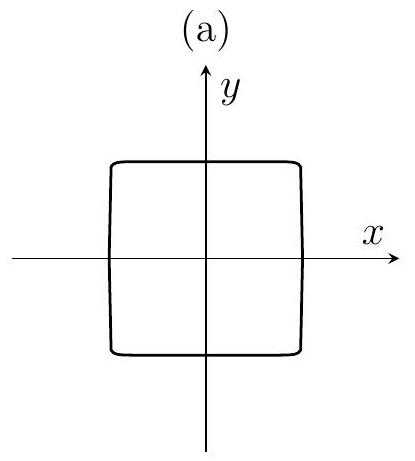
\includegraphics[max width=\textwidth]{2024_03_31_cf7383a5f8d68fb42455g-06(4)}
\end{center}

(b)

\begin{center}
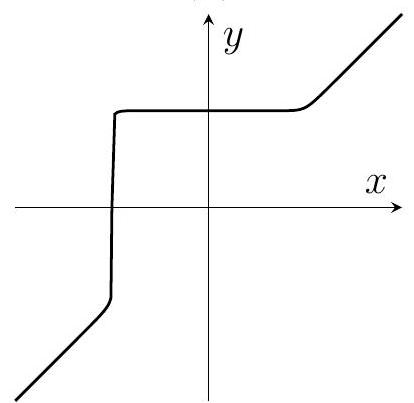
\includegraphics[max width=\textwidth]{2024_03_31_cf7383a5f8d68fb42455g-06}
\end{center}

(c)

\begin{center}
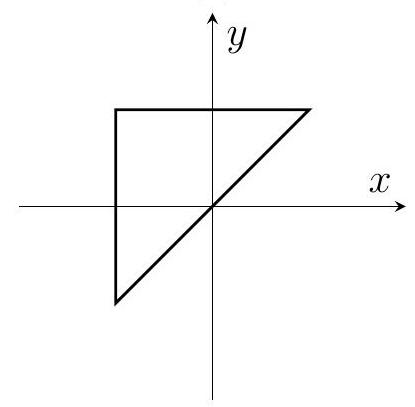
\includegraphics[max width=\textwidth]{2024_03_31_cf7383a5f8d68fb42455g-06(2)}
\end{center}

(d)

\begin{center}
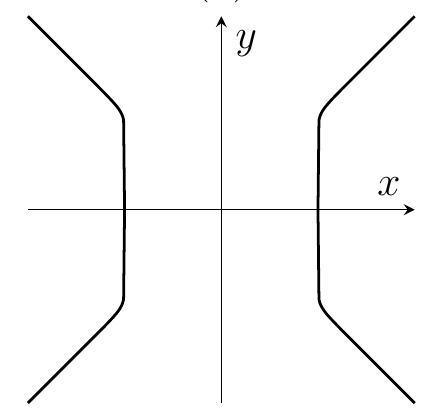
\includegraphics[max width=\textwidth]{2024_03_31_cf7383a5f8d68fb42455g-06(3)}
\end{center}

(e)

\begin{center}
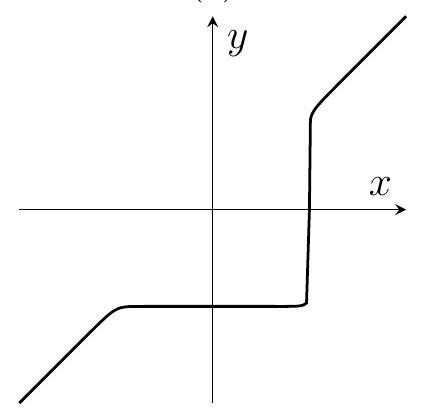
\includegraphics[max width=\textwidth]{2024_03_31_cf7383a5f8d68fb42455g-06(1)}
\end{center}

F. The following are statements about a real number $x$.

$$
P: \quad \frac{x^{2}-1}{x+2}<0, \quad Q: \quad \frac{1+x}{1-x}>0 .
$$

Then it follows that

(a) $P$ implies $Q$ but $Q$ does not imply $P$.

(b) $Q$ implies $P$ but $P$ does not imply $Q$.

(c) $P$ and $Q$ are equivalent.

(d) If $P$ is true then $Q$ is false.

(e) If $Q$ is true then $P$ is false.

G. The functions $S$ and $T$ are defined by

$$
S(x)=x+1, \quad T(x)=\frac{1}{2} x-1 .
$$

Beginning with $x=0$ the functions $S$ and $T$ are repeatedly applied in some order. For example, $\operatorname{SST} S(0)=\frac{3}{2}$. The set of possible outputs is

(a) all positive rational numbers.

(b) all rational numbers greater than -1 with denominator a power of 2 when written in lowest terms.

(c) all rational numbers with denominator a power of 2 when written in lowest terms.

(d) all positive rational numbers with denominator a power of 2 when written in lowest terms.

(e) all rational numbers greater than -2 with denominator a power of 2 when written in lowest terms.

H. A sequence $a_{n}$ is defined by $a_{0}=A$ and $a_{k}=\left(a_{k-1}\right)^{2}$ for $k>0$, where $A>1$. The sequence $b_{n}$ is defined by $b_{n}=\log _{2} a_{n}$. The sequence $b_{n}$ is

(a) constant

(b) an arithmetic progression

(c) a geometric progression

(d) all of the above

(e) none of the above

I. An equilateral triangle is drawn in the $x y$-plane. Two of its vertices are at $(0,0)$ and $(1000,0)$. The number of points $(x, y)$ inside the triangle, where $x$ and $y$ are both whole numbers, equals\\
(a) 866,025 ,\\
(b) 866,026 ,\\
(c) 866,027 ,\\
(d) 432,512 ,\\
(e) 432,513 .

[Note that $\sqrt{3}=1.7321$ to 4 decimal places.]

J. Let $R$ be the region where all four of the following inequalities hold

$$
x^{2}<2+y, \quad x^{2}<2-y, \quad y^{2}<2+x, \quad y^{2}<2-x
$$

What is the area of $R$ ?\\
(a) 0 ,\\
(b) $\frac{28}{3}$,\\
(c) $4+2 \pi$,\\
(d) $\frac{4}{3}(8 \sqrt{2}-7)$,\\
(e) infinite.


\end{document}